%%%%%%%%%%%%%%%%%%%%%%%%%%%%%%%%%%%%%%%%%%%%%%%%%%%%%%%%%%%%%%%%%%%%%%%%%%%%%%%%
%2345678901234567890123456789012345678901234567890123456789012345678901234567890
%        1         2         3         4         5         6         7         8

\documentclass[letterpaper, 10 pt, conference]{ieeeconf}  % Comment this line out if you need a4paper

%\documentclass[a4paper, 10pt, conference]{ieeeconf}      % Use this line for a4 paper

\IEEEoverridecommandlockouts                              % This command is only needed if 
                                                          % you want to use the \thanks command

\overrideIEEEmargins                                      % Needed to meet printer requirements.

% The following packages can be found on http:\\www.ctan.org
\usepackage{graphics} % for pdf, bitmapped graphics files
\usepackage{amsmath} % assumes amsmath package installed
\usepackage{amssymb}  % assumes amsmath package installed
\usepackage[font=small]{subcaption}
\usepackage{graphicx}
\usepackage{hyperref}
\usepackage[lined,commentsnumbered]{algorithm2e}
\usepackage{algorithmic}
\usepackage{xfrac} %\sfrac
\usepackage{enumerate}

\newtheorem{theorem}{\bf Theorem}
\newtheorem{todo}{\bf Todo}
\newtheorem{remark}{\bf Remark}
\newtheorem{corollary}{\bf Corollary}
\newtheorem{definition}{\bf Definition}
\newtheorem{lemma}{\bf Lemma}
\newtheorem{proposition}[theorem]{\bf Proposition}

\captionsetup{font=small, labelfont=bf}

\title{\LARGE \bf
Periodic Trajectories of Mobile Robots}


\author{Alexandra Q. Nilles, Israel Becerra and Steven M. LaValle% <-this % stops a space
\thanks{A. Nilles, I. Becerra and S. M. LaValle are with the Department of Computer Science, 
University of Illinois at Urbana-Champaign. Urbana, IL 61801, USA. 
        {\tt\small \{nilles2,israelb4,lavalle\}@illinois.edu}}%
}


\begin{document}



\maketitle
\thispagestyle{empty}
\pagestyle{empty}


%%%%%%%%%%%%%%%%%%%%%%%%%%%%%%%%%%%%%%%%%%%%%%%%%%%%%%%%%%%%%%%%%%%%%%%%%%%%%%%%
\begin{abstract}


Differential drive robots, such as robotic vacuums, often
have at least two motion primitives: the ability to travel forward in straight
lines, and rotate in place upon encountering a boundary. They are often equipped
with simple sensors such as contact sensors or range finders, which allow them
to measure and control their heading angle with respect to environment
boundaries.
We aim to find minimal control schemes for creating stable, periodic
``patrolling" dynamics for robots that drive in straight lines and ``bounce" off
boundaries at
controllable angles. As a first step toward analyzing high-level mobile robot
dynamics in more general environments, we analyze the location and stability of
periodic orbits in regular polygons.
The contributions of this paper are:
1) proving the existence of periodic trajectories in n-sided regular polygons
and showing the range of bounce angles that will produce such trajectories;
2) an analysis of their stability and robustness to
modeling errors; and
3) a closed form solution for the points where the robot
collides with the environment boundary while patrolling.
We present simulations confirming our theoretical results.

\end{abstract}


%%%%%%%%%%%%%%%%%%%%%%%%%%%%%%%%%%%%%%%%%%%%%%%%%%%%%%%%%%%%%%%%%%%%%%%%%%%%%%%%
\section{INTRODUCTION}

Consider the path that a differential-drive mobile robot takes as it navigates a room.
This robot has two motion primitives that it can execute reliably: moving in a straight
line and turning in place. We can equip the robot with sensors that allow it to
determine whether it is in contact with an environmental boundary and measure
its heading relative to that boundary.

The main question addressed by this work is: \textit{can we guarantee that the robot 
\textbf{patrols} a space on a repeatable, periodic path?} If so, what are the
 sensing and actuation requirements of this task? A better understanding of
this common robotic task could lead to robots that are robust in the face of
noise and complicated environments. Robots with
robust patrolling behavior have applications such as
monitoring environmental conditions in labs, warehouses, or greenhouses, where
a few fixed sensors may not give adequate information.

Existing techniques for producing repeatable motion patterns for mobile robots
involve equipping the robots with high-resolution sensors such as cameras, and
using algorithms such as simultaneous localization and mapping (SLAM) to compute
a map of the space and estimate the robot's state
\cite{slamSolution,fastslam,durrant2006}. However, these robots can be
expensive, require a large amount of computational and electrical power, and
their accuracy can be impacted by changing environmental conditions (such as low
light). In situations which require high-resolution mapping and localization in
dynamic environments these tradeoffs are clearly worthwile. However,
tasks such as monitoring humidity or temperature in a warehouse require only
repeatable orbits in a relatively simple space, and some guarantees about what parts of the space
will be covered. Robots with minimal sensing, actuation and control requirements
will be more reliable and efficient at such tasks. Our approach requires 
precise knowledge about the structure of the environment, but does not require
observation or calculation of the exact position of the robot. Such tradeoffs
are common in robots, and allow us to optimize robotic designs for specific
tasks and constraints.

The key approach of this work is treating the robot
as a dynamical system defined
by its motion primitives, independent of the hardware implementation.
The contributions of this paper are 1) proving the existence of
periodic orbits in $n$-sided regular polygons, and showing the range of bounce
angles that will produce periodic orbits;
2) an analysis of these orbits, showing their stability and robustness; and 3) 
an analytic solution of the locations where the robot collides with the
environment while in these orbits.

\begin{figure}[tp]
\begin{subfigure}{.25\textwidth}
\centering
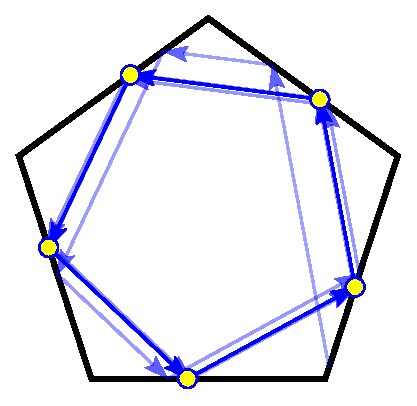
\includegraphics[width=0.8\linewidth]{../figs/pent_05rad.pdf}
\captionof{figure}{\sffamily\footnotesize$\theta = 1.07$ rad, 20
bounces. \label{0.5rad}}
\end{subfigure}%
\begin{subfigure}{0.25\textwidth}
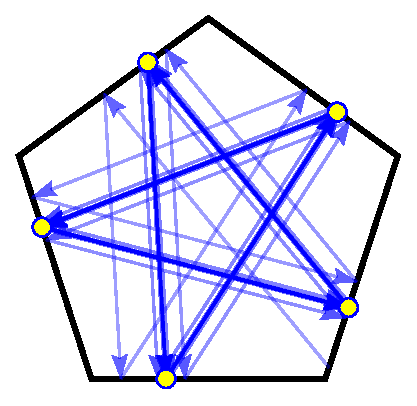
\includegraphics[width=0.8\linewidth]{../figs/pent_1rad.pdf}
\captionof{figure}{\sffamily\footnotesize $\theta = 0.57$ rad, 50
bounces. \label{0.57rad}}
\end{subfigure}
\begin{subfigure}{0.25\textwidth}
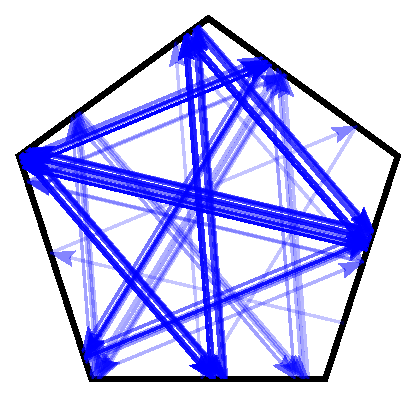
\includegraphics[width=0.8\linewidth]{../figs/pent_165rad.pdf}
\captionof{figure}{\sffamily\footnotesize$\theta = -0.08$ rad, 75
bounces. \label{1.65rad}}
\end{subfigure}%
\begin{subfigure}{0.25\textwidth}
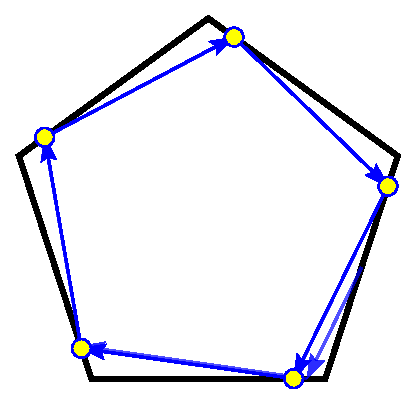
\includegraphics[width=0.8\linewidth]{../figs/pent_3rad.pdf}
\captionof{figure}{\sffamily\footnotesize$\theta = -1.4$ rad, 20
bounces. \label{3.0rad}}
\end{subfigure}
\caption{Different behaviors of bounce trajectories in a regular pentagon.
Older bounces become 2\% more transparent with each new bounce. The circle on
the boundary indicates the starting point of the trajectory. Figure (c) shows
that periodic orbits are not guaranteed for all bounce angles.}
\end{figure}

This paper is organized as follows: Section \ref{related} describes related work.
Section \ref{model} presents the model definition and
some useful concepts from dynamical systems. Section \ref{adj_edge} analyzes the 
case where the robot is constrained to bounce between sequential edges of the
polygon, and we prove the existence and location of a periodic path using a
fixed point technique.
Section \ref{general} generalizes this approach to find periodic paths of period $k$ in
regular $n$-gons, when $k$ divides $n$. Section \ref{conclusion} discusses possible extensions
of this work, including to more generalized polygonal environments, and
remaining open questions. By providing strong guarantees in the case of regular
polygonal environments, we hope to lay the groundwork for analysis of more
complex environments. 


\section{RELATED WORK\label{related}} 

This dynamical system is closely related to mathematical billiards
\cite{billiards}. In billiards, an agent travels in a straight line until
contacting a boundary of its environment, then bounces so that the incident
angle is related to the outgoing angle by $\theta_{o} = -\theta_{i}$
(\textit{specular} bouncing, such as how a laser beam
reflects off mirrors). Our system
generalizes this model by allowing the robot to control the angle of reflection.

There has been significant progress in generalizations of the billiards model: for example, 
\textit{pinball billiards} is a model where the agent is deflected toward the
normal with each bounce, $\theta_{o} = - \gamma \theta_{i}$ for
$0 \leq \gamma \leq 1$. If the agent always bounces at the normal vector
($\gamma = 0$), this is called \textit{slap billiards}. Work in this area focuses on
analyzing the existence and structure of attractors \cite{pinball} \cite{DelMagno2014}.
Additionally, \cite{Jones1998} looks at the knots formed by periodic billiards
in rectangular prisms. They generalize
the idea of a constant-angle bounce to
three dimensions, motivated by the behavior of Paramecium. They show that knots
formed by constant bounces of $\pi/4$ in a rectangular prism are equivalent to
billiard knots in a cube. Our study is in two dimensions and focuses on the
necessary conditions for periodic orbits.

We are also inspired by work on map dynamics in polygons such as
\cite{schwartz_billiards} and \cite{schwartz1992}. Also related is work on the
combinatorial complexity of the region visited
by specular bouncing (``visibility with reflection") in simple polygons
\cite{Aronov1996}. There, the authors show the combinatorial complexity of the
region touched after $k$ bounces and provide a near-optimal algorithm for
computing the region. Our work differs by analyzing non-specular bouncing and
the effects of environment geometry. Specifically, we focus on determining
regions of minimal complexity.

In \cite{nakamura2001chaotic}, the authors describe a
controller which generates chaotic dynamics in the heading of a mobile robot,
guaranteeing that it will scan an entire connected workpace.
Similarly to this work, their implementation requires a measurement of
the local normal of boundaries upon contact. While the underlying dynamics are
different, this work also treats the robot as a dynamical system over
the workspace and leverages the results for useful patrolling behavior.

The motion primitives described in this paper are feasibly implemented on
actual robots - in \cite{LewOKa13}, the authors describe a differential-drive robot with bump and infrared
range sensors
which executes the same type of ``bounces" described in this paper with error less
than $\pm 10^{\circ}$. In that work, the authors developed an algorithm for navigation with such a
robot; similarly,
we show that patrolling is possible, and provide bounds on how much noise can be
tolerated. Similarly, wall following robots \cite{Carelli2003,Lamp05} are often capable of the
motion primitives we describe - this work could help extend the capabilities of such
robots with new motion strategies for patrolling the interior of a space.

\subsection{Prior Work}

In \cite{bounce}, the authors
characterized some of the long-term dynamics of this dynamical system. They
showed that the robot will have an orbit of period two between parallel edges,
and the robot will move monotonically ``outward" from acute vertices or edges
that would meet in an acute vertex if extended to their intersection.

The authors in \cite{bounce} defined distance- and link-unbounded
segments as regions of the boundary where the robot may
travel an unbounded distance or bounce an unbounded number of times. That work describes an algorithm for classifying the
 boundary of an arbitrary polygon into distance- and link-unbounded segments. 
 However, the algorithm will not terminate when the robot's trajectory converges 
 to a periodic orbit, since in this case the distance- and link-unbounded regions shrink to points on the polygon boundary, such as in Figures \ref{0.5rad} and \ref{0.57rad}.

One purpose of this paper is to begin to identify cases where the dynamical system's attractor is a set of separate points, not intervals, on
the environment boundary. The
algorithm in \cite{bounce} can be used only for environments with attractors that are
segments on the boundary, for which the algorithm is guaranteed to terminate.


\section{MODEL DEFINITION\label{model}}

A point robot moves in a bounded subset of the plane $P$,
defined by a continuous boundary $\delta P$. For most 
of this discussion, the environment will be a simple regular polygon, so $\delta P$ 
is an $n$-gon with $n$ straight edges intersecting at $n$ vertices
$(v_0, v_1, \ldots, v_{n-1})$.  An edge of the polygon is represented as $v_i
v_{i+1}$.

The robot drives in a straight line until encountering $\delta P$. It then rotates
until its heading is at an angle $\theta$ clockwise of the inward-facing boundary
normal, where $-\pi/2 < \theta < \pi/2$. Then the robot repeats this procedure
indefinitely. Figure \ref{bounce_def} shows two sample bounces, at
angles $\theta^+$ and $\theta^-$.

\begin{figure}[thpb]
  \centering
  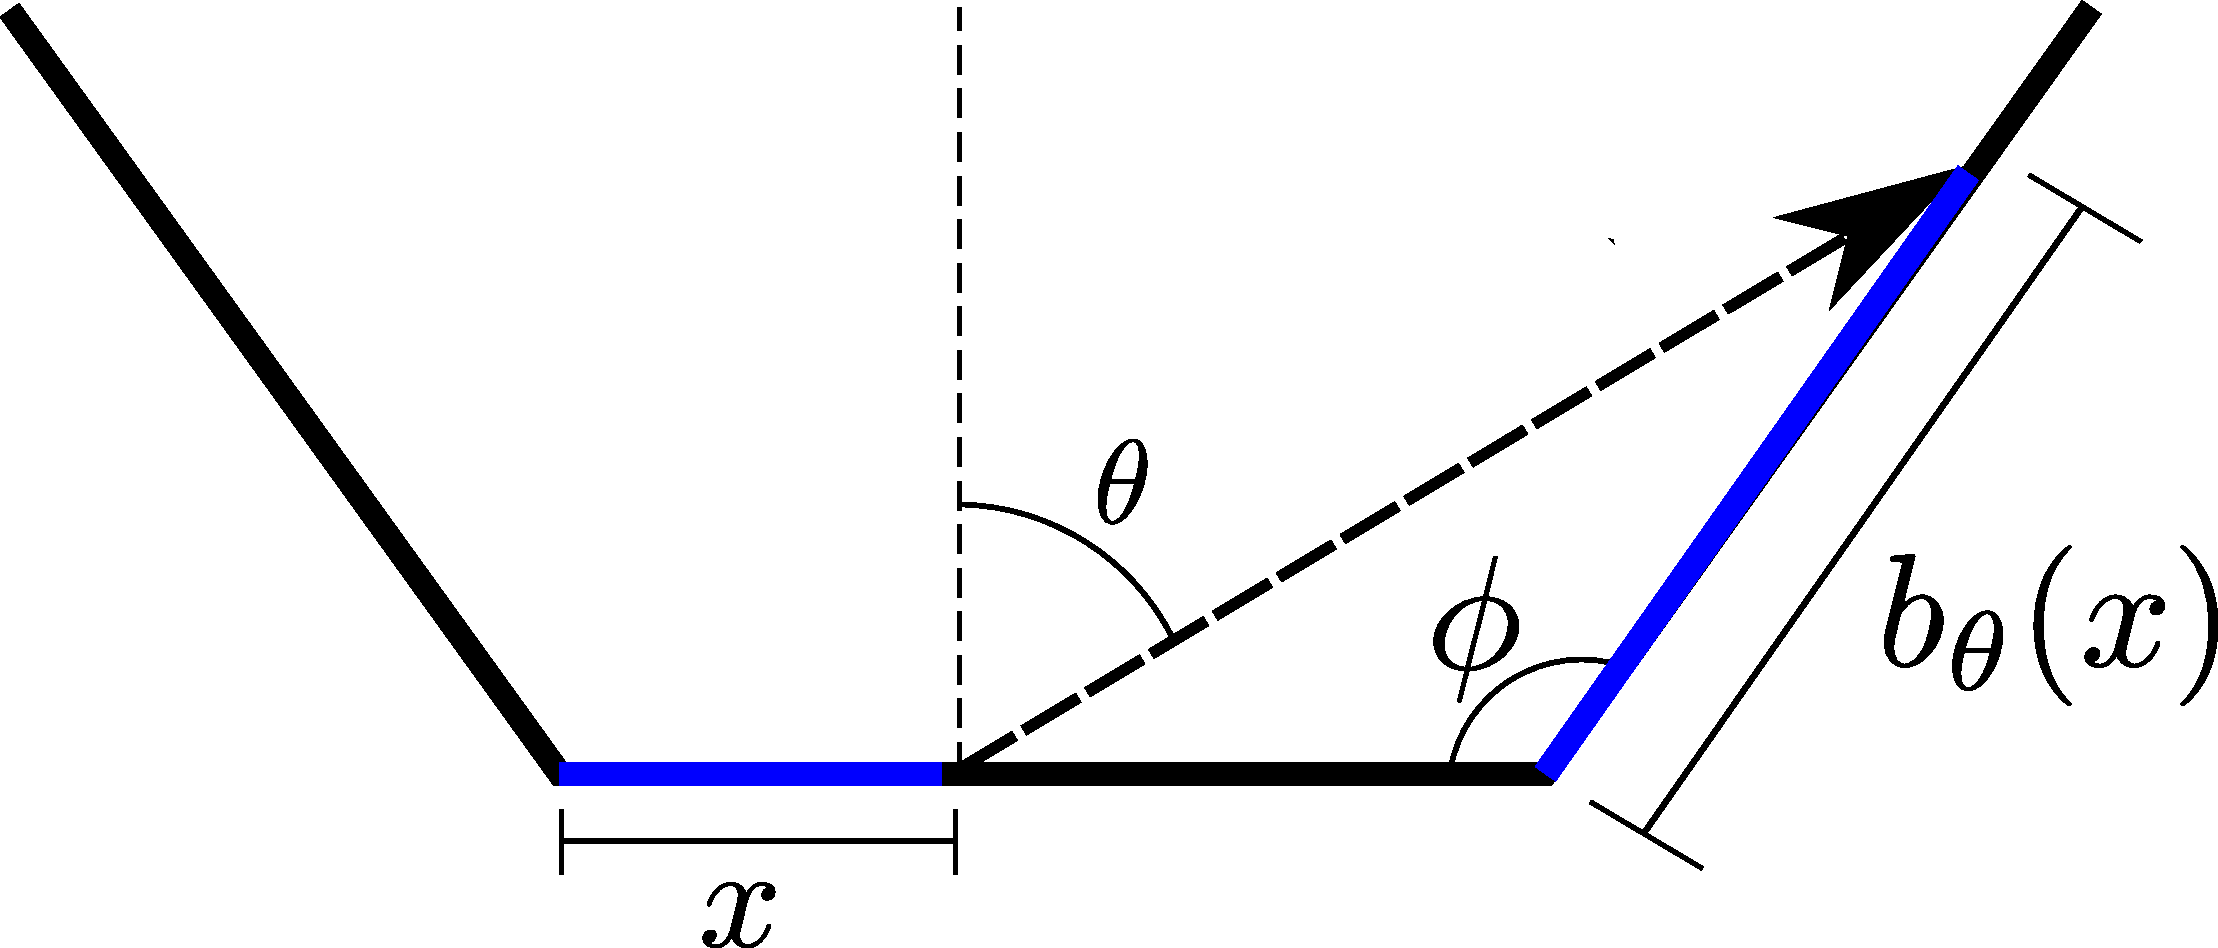
\includegraphics[width=0.4\textwidth]{../figs/simple_bounce_def.pdf}
  \caption{A sample bounce, showing $\theta$ measured clockwise from the normal. The other labels show the geometric meaning of the
    bounce map defined in Lemma \ref{Lemma:1}.}
  \label{bounce_def}
\end{figure}

The function that these actions define between points
on $\delta P$ is $B_{\theta}: \delta P \to \delta P$, defining our dynamical system.
We will refer to this function as the \textit{bounce map}, in the same spirit as
the \textit{logistic map} in discrete dynamical systems, not to be confused with
a map of the environment.
When the bounce map is iterated $k$ times, we write $B^k_{\theta}$.
$B_{\theta}$ is not well defined
on vertices of $\delta P$, so we will not consider trajectories which reach a
vertex.

A sequence of points $[p_0, \ldots, p_k]$ is a \textit{flow} of $B_{\theta}$ if
$p_i = B_{\theta}(p_{i-1})$ for $1 \leq i \leq k$. A flow is an \textit{orbit}
with \textit{period} $k$ if $B_{\theta}(p_{k-1}) = p_0$. A \textit{limit
cycle} is an orbit where nearby flows tend asymptotically toward or away from
the orbit \cite{jackson1992}.

\section{BOUNCING TO ADJACENT EDGE\label{adj_edge}}
\label{section:BAE}

Take a regular $n$-gon with boundary $\delta P$, each side of length $l$, and
each interior angle of $\phi = (n - 2)\pi/n$ radians \cite{johnson1929}. In simulation, for some values of $\theta$ we observe
stable orbits that bounce off each adjacent edge (Figure \ref{0.5rad}). 
To analyze these orbits, we imagine that $B_{\theta}$ is
constrained to send the robot from edge $v_i v_{i+1}$ to edge $v_{i+1} v_{i+2}$
for all bounces, and then solve for the conditions necessary to guarantee this
behaviour. 

We begin our analysis by presenting a trigonometric function
(Lemma~\ref{Lemma:1}) that is used to determine the existence and location of a
periodic path. Lemma~\ref{Lemma:2} establishes the conditions under which
that function is a contraction mapping with a unique fixed point. A fixed point
of this mapping function corresponds to a stable orbit that has the shape of a
regular $n$-gon, inscribed in $\delta P$. Finally,
Proposition~\ref{Proposition:1} presents a closed form solution for the fixed
point that allows us to locate where the robot collides with the polygon in
these stable orbits.

\begin{lemma} \label{Lemma:1}
Assume that the robot bounces at angle $\theta$ to the next adjacent edge in a
counterclockwise (positive) direction. Under this condition, define the constrained bounce
map $b^+_{\theta} : (0, l) \to (0, l)$ which takes $x$, the
robot's distance from vertex $v_i$, and maps it to $b^+_{\theta}(x)$,
the resulting distance from vertex $v_{i+1}$. This mapping function is given by
\begin{equation} \label{b-one-bounce}
b^+_{\theta}(x) = c(\theta)(l-x),
\end{equation}
in which $c(\theta) = cos(\theta) / cos(\theta - \phi)$.
\end{lemma}
\begin{proof}
Using the triangle formed by two adjacent edges and the robot's trajectory
between them (see Fig \ref{bounce_def}), we can solve for $b^+_{\theta}$.
The law of sines establishes that
$$ \frac{b^+_{\theta}(x)}{\sin (\pi/2-\theta)} = \frac{l-x}{\sin
(\pi-(\pi/2-\theta)-\phi)} $$

\noindent which we can rewrite as
$$ b^+_{\theta}(x) = \frac{\cos(\theta)}{\cos
(\theta-\phi)}(l-x)  = c(\theta) (l-x). $$

\end{proof}

\begin{lemma} \label{Lemma:2}
If $|c(\theta)| < 1$, then $b^+_{\theta}(x)$ is a contraction
mapping and has a unique fixed point.
\end{lemma}
\begin{proof}
We take $(0,l)$ to be a metric space with metric $d(x,y) =
|y-x|$. To be a contraction mapping, $b^+_{\theta}$ must satisfy

$$ d(b^+_{\theta}(x), b^+_{\theta}(y)) \leq k d(x,y) $$

for all $x, y \in (0,l)$ and some nonnegative real number $0 \leq k < 1$.

When we check this property, we see that
\begin{align*}
d(b^+_{\theta}(x), b^+_{\theta}(y)) & = | c(\theta)(l-y) - c(\theta)(l-x)| \\
                               & = | c(\theta) (x-y) | \\
                               & = | c(\theta) | d(x,y).
\end{align*}

Thus if $|c(\theta)| < 1$, then $b^+_{\theta}$ is a contraction mapping, and by the Banach fixed-point
theorem, it has a unique fixed point \cite{Granas2003}.
\end{proof}
\begin{corollary} \label{corollary:sp}
At the fixed point, $b^+_{\theta}$ represents the 
robot bouncing from a point that is distance $x_{FP}$ from vertex $v_i$, to a
point that is distance $x_{FP}$ from vertex $v_{(i+1) \text{mod }n}$, for all $i \in
[0,\ldots, n-1]$.
Thus, a fixed point of $b^+_{\theta}$ implies an orbit of $B_\theta$.


\end{corollary}
\begin{remark} \label{rm1}
Note that the proof of Lemma~\ref{Lemma:2} holds for all $x,y \in
(0, l)$, so it does not matter where the robot starts bouncing,
implying that this orbit is a stable limit cycle of the dynamical system, 
with the largest possible region of stability.
\end{remark}

\begin{proposition} \label{Proposition:1}
In every regular $n$-sided polygon with side
length $l$ and interior angle $\phi$, there exists a range for $\theta$ such
that iterating $B_{\theta}(x)$ on any $x \in \delta P$ results in a stable limit
cycle of period $n$, which strikes the boundary at points that are distance $x_{FP}$
from the nearest clockwise vertex. $x_{FP}$ is given by

\begin{equation}
x_{FP} = 
\begin{cases}
        \frac{l c(\theta)}{1 + c(\theta)} & \phi/2 < \theta
< \pi/2 \\
        \frac{l}{1+c(\theta)} & -\pi/2 < \theta
< -\phi/2
\end{cases}
\end{equation}

\noindent in which $c(\theta) = cos(\theta) / cos(\theta - \phi)$.

\end{proposition}
\begin{proof}
In a regular $n$-sided polygon with side length $l$, let the robot begin its
trajectory at a point $p \in P$ which is at a distance $x$ from the nearest
vertex in the clockwise direction. We will begin by constraining the robot to
bounce counterclockwise, at an angle $0 < \theta < \pi/2$ 
such that it strikes the nearest
adjacent edge, such as in Figure \ref{0.5rad}. The function $b^+_{\theta}$ 
given in Lemma~\ref{Lemma:1} describes such bouncing behaviour.

By Lemma~\ref{Lemma:2}, $b^+_{\theta}(x)$ has a unique fixed point, which is
an orbit of $B_\theta$ since the
robot is contacting each edge at the same distance from the
vertex at each bounce. By iterating the map $b^+_{\theta}$,
we can explicitly find the value of
the fixed point, and thus the points on $\delta P$ touched by the
robot in its orbit. Iterating $b^+_{\theta}$ $k$ times yields

\begin{align*}
{b^+_{\theta}}^k(x) & = c(\theta) (l-c(\theta)(l- \ldots c(\theta)(l-x) \ldots )) \\
                & = \sum_{i=1}^{k} (-l) (-c(\theta))^i + (-c(\theta))^kx 
\end{align*}

\noindent and taking the limit as $k \to \infty$ and shifting the index gives
\begin{equation*}
{b^+_{\theta}}^\infty(x) = l + \sum\limits_{i=0}^\infty (-l)(-c(\theta))^i
\end{equation*}
.

Note that the starting position, $x$, drops out when the limit
is taken - the orbit converges regardless of
starting position. The sum is geometric, and since $|c(\theta)| < 1$ 
(the condition stated in Lemma~\ref{Lemma:2}), the fixed point 
(for counterclockwise orbits) becomes

\begin{equation*}
(b^+_{\theta})^\infty(x) = \frac{lc(\theta)}{1+c(\theta)}
\end{equation*}
.

So the trajectory of a robot with bounce angle $\theta$ satisfying
$|c(\theta)| < 1$ converges to a limit cycle in the shape of an inscribed
$n$-gon, with collision points $x_{FP}$ at distance $(lc(\theta))/(1+c(\theta))$
from the nearest vertex in the clockwise direction. When this calculation is
redone for bounces in the counterclockwise direction ($-\pi/2 < \theta < 0$), the resulting fixed point
$x_{FP}$ is $l/(1 + c(\theta))$. Moreover, since $c(\theta) \in (0, 1)$ 
for stable orbits, and considering the past two
expressions for $x_{FP}$, we find that the fixed point $x_{FP}$ for bounces can
take all values in $(0, l)$ except for $l/2$, which would require
$c(\theta) = 1$.

Next, we examine the stability condition,
$|\frac{\cos(\theta)}{\cos(\theta-\phi)}| < 1$. 
Since $0 < \theta < \pi/2$ for $b^+_{\theta}$, $\cos(\theta)$ is always
positive, then we must have $|\cos(\theta-\phi)| > \cos(\theta)$, from where we 
can obtain the range $\phi/2 < \theta < \pi/2$. Likewise, in the clockwise 
direction, $-\pi/2 < \theta < 0$ yields $-\pi/2 <
\theta < -\phi/2$. Thus, we have a guarantee on the range of bounce angles that
will result in periodic orbits, starting from any point on the polygon's
boundary.
\end{proof}

\begin{remark}
Note that calculating the Lyapunov exponent \cite{jackson1992} for the map $b_{\theta}(x)$
gives the same result: $|db_{\theta}(x)/dx| = |c(\theta)|$, which implies that
$|c(\theta)| < 1$ gives a stable fixed point.
\end{remark}

\begin{figure}[th]
\begin{subfigure}{.25\textwidth}
\centering

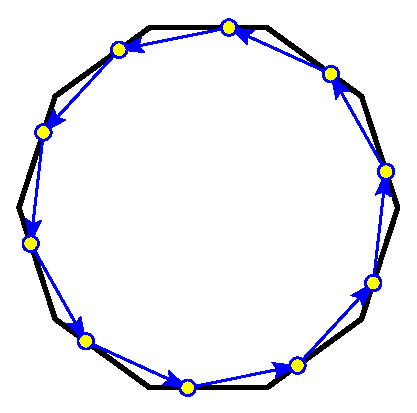
\includegraphics[width=0.7\linewidth]{../figs/dec_limit_0pt2.pdf}

\end{subfigure}%
\begin{subfigure}{0.25\textwidth}

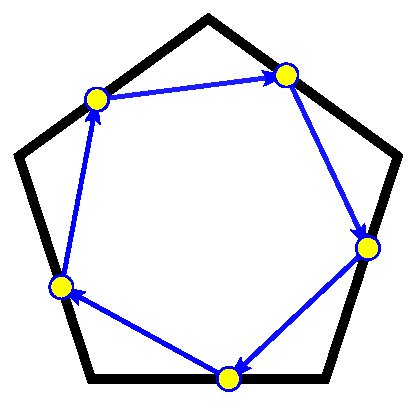
\includegraphics[width=0.7\linewidth]{../figs/pent_limit_0pt5.pdf}

\end{subfigure}

\caption{Simulated orbits for adjacent edge bouncing in
regular polygons. Predicted collision points are indicated by circles. Both simulations are of the trajectory after 300 bounces
from an arbitrary start point. \label{prediction}}
\end{figure}



\section{GENERALIZATION}
\label{general}

Instead of bouncing between adjacent edges, we may ask what happens 
when the robot bounces between edge $v_0 v_1$ and edge $v_m v_{m+1}$, 
``skipping" $m-1$ edges, such as in Figure \ref{0.57rad} where the robot bounces off 
every other edge.

Proposition~\ref{Proposition:2} states the existence of a stable limit cycle
with period $k$ in every regular $n$-sided polygon, in the particular case where
$k|n$. Then, following a similar approach as in Section~\ref{section:BAE}, we
prove in Lemma~\ref{Lemma:4} that the trigonometric function of
Lemma~\ref{Lemma:3} is a contraction mapping with a unique fixed point, and
conclude with Theorem~\ref{Theorem:1} presenting a closed form solution for the
fixed point (hence the location of the stable orbit) when the robot bounces
skipping $m-1$ edges.

\begin{proposition} \label{Proposition:2}
In every regular $n$-sided polygon, there
exists a stable limit cycle with period $k$ for all $k$ such that
$k > 2$ and $k|n$.
\end{proposition}
\begin{proof}
For all prime $n\geq3$, the statement
is true by Proposition~\ref{Proposition:1}, since $k=n$ for $k|n$, 
and Proposition~\ref{Proposition:1} guarantees a stable limit 
cycle that strikes each edge sequentially.

Now consider any non-prime $n>3$, and assume $k>2$ to avoid
trajectories between parallel edges (addressed in \cite{bounce}).
Proposition~\ref{Proposition:1} guarantees a stable limit cycle that strikes each
edge of an $n$-sided polygon sequentially. For all $k$ such that
$k|n$, we can choose $k$ edges of the $n$-gon such that the
edges are equally spaced. We can then imagine extending
these edges to their intersection points, forming a regular $k$-gon. 
By Proposition~\ref{Proposition:1}, the bounce map in this regular $k$-gon
is guaranteed to induce a stable limit cycle, with collision
points at parameter $x_{FP}$ on the edge for all $x_{FP}$ except the very
center point of the edge. Thus $\theta$ can be chosen such that the
bounce map sends the robot to every $(n/k)$- \textit{th} edge such
that the trajectory will converge to a stable cycle with period
$k$. The result follows.
\end{proof}

\begin{figure}[bh]
\centering
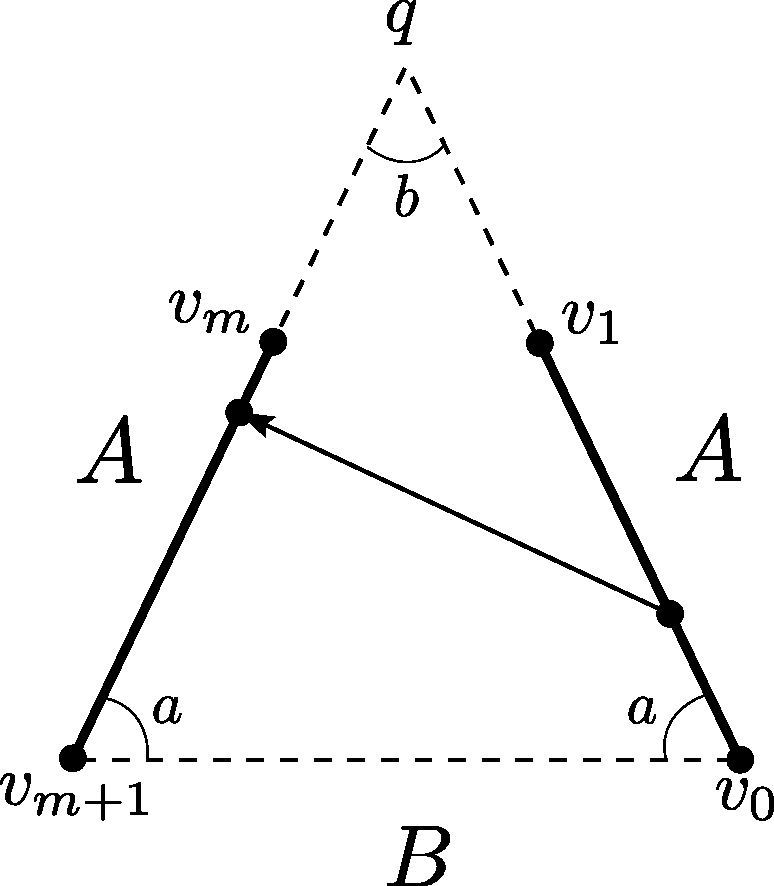
\includegraphics[width=0.2\textwidth]{../figs/gen_bounce.pdf}
\captionof{figure}{A bounce from edge $v_0v_1$ to edge $v_mv_{m+1}$. The other
edges of the polygon are not drawn, and the distance between the edges is not to scale.
\label{gen_bounce}}
\end{figure}

\begin{lemma} \label{Lemma:3}

Assume that $B_{\theta}$ is constrained so the robot ``skips" $m-1$ edges with
each bounce in a counterclockwise direction. This constrained bounce
map $b^+_{\theta,m} : (0, l) \to (0, l)$, which takes $x$ (the
robot's distance from vertex $v_i$) and maps it to $b^+_{\theta,m}(x)$
(the resulting distance from vertex $v_{i+m}$) is given by

\begin{equation} \label{b-one-bounce}
b^+_{\theta,m}(x) = c(\theta)(A-x) + l - A,
\end{equation}

%\begin{equation} \label{b-one-bounce}
%b_{\theta,m}(x) =
%\begin{cases}
%        c(\theta)(A-x) + l - A,  & \frac{\phi_m}{2} < \theta <
%\frac{\phi_{m-1}}{2} \\
%        c(\theta)(l-A-x) - A, & \frac{-\phi_{m-1}}{2} < \theta <
%\frac{-\phi_m}{2}
%\end{cases}
%\end{equation}

\noindent in which $c(\theta)$ is generalized to

\begin{equation} \label{equation:c_theta}
c(\theta) = \cos(\theta)/\cos \left(\theta - \frac{\pi(n-2m)}{n}\right)
\end{equation}

\noindent and

\begin{equation} \label{equation:A}
A = \frac{l \sin(\frac{\pi(m+1)}{n}) \sin( \frac{m \pi}{n} )}{ \sin(
\frac{\pi}{n} ) \sin( \frac{\pi(n-2m)}{n} ) } .
\end{equation}

%\noindent and
%
%\begin{equation} \label{equation:phi}
%\phi_m = \frac{\pi(n-2m)}{n}
%\end{equation}
\end{lemma}

\begin{proof}
Let $m \leq \lfloor n/2 \rfloor$ - the robot bounces counterclockwise.
Without loss of generality assume that we start on edge $v_0 v_1$.
Extend the line segments $v_0 v_1$ and $v_m v_{m+1}$ to their point of
intersection $q$, forming the triangle $v_0 v_{m+1} q$. Let $a = \angle q
v_{m+1} v_0 = \angle q v_0 v_{m+1}$, by symmetry. Let $b = \angle v_{m+1} q
v_0$. Let $A = |q v_{m+1}| = |q v_0|$ and $B = |v_{m+1} v_0|$ (see Figure
\ref{gen_bounce}). Each of the sides of the polygon has length $l$, and the robot
begins its trajectory at a point which is distance $x$ from $v_0$. We wish to
find $b^+_{\theta,m}(x)$, the distance from the endpoint of the bounce to point
$v_m$.

By the law of sines, we have

$$ A = \frac{B \sin(a)}{\sin(b)} $$

\noindent We can then form the triangle from the points $v_0$, $v_{m+1}$, and the center
of the regular $n$-gon. The distance from the center of a regular $n$-gon to any
of its vertices is $\frac{l}{2 \sin(\pi/n)}$ \cite{johnson1929}. The angle subtended
by the edges $v_0 v_1$ through $v_m v_{m+1}$ is $2 \pi (m+1)/n$. Thus, $B$
becomes

$$ B = \frac{l \sin( \pi (m+1) /n)}{\sin (\pi / n)} $$.

The angle $a$ can be found by considering the polygon formed by edges $v_0 v_1$
through $v_m v_{m+1}$, closed by edge $v_{m+1} v_0$. This polygon has $m+2$
vertices, so its angle sum is $m \pi$. $m$ of these vertices have the vertex
angle of the regular $n$-gon, $(n-2) \pi /n$. The remaining two vertices have
angle $a$. Therefore, $2a + m(n-2)\pi/n = m \pi$, so $a = m \pi / n$, and thus 

$$ A = \frac{l \sin(\frac{\pi(m+1)}{n}) \sin( \frac{m \pi}{n} )}{ \sin(
\frac{\pi}{n} ) \sin( \frac{\pi(n-2m)}{n} ) } $$.

Using the triangle formed by the the bounce of the robot and vertex $q$,
the law of sines states

$$ \frac{A-x}{\sin( \theta - \pi/2 + (2 \pi m)/n )} = \frac{ A - l +
b^+_{\theta,m}(x)}{sin(\pi/2 - \theta)}, $$

\noindent which we rewrite as

\begin{align*}
b^+_{\theta,m}(x) & =\frac{(A-x) \cos(\theta)}{\cos(\theta - \frac{\pi
(n-2m)}{n})} + l -A \\ \\
                & = c(\theta)(A-x)  + l -A. \\
\end{align*}
\end{proof}


\begin{lemma} \label{Lemma:4}
If $|c(\theta)| < 1$, then $b^+_{\theta,m}(x)$ is a contraction
mapping, and therefore has a unique fixed point.
\end{lemma}
\begin{proof}
We take $(0,l)$ to be a metric space with metric $d(x,y) =
|y-x|$. To be a contraction mapping, $b^+_{\theta,m}$ must satisfy
\begin{equation*}
d(b^+_{\theta,m}(x), b^+_{\theta,m}(y)) \leq k d(x,y) 
\end{equation*}
\noindent for all $x, y \in (0,l)$ and some nonnegative real number $0 \leq k < 1$.

When we check this property, we see that
\begin{align*}
d(b^+_{\theta,m}(x), b^+_{\theta,m}(y)) & = | b^+_{\theta,m}(x) - b^+_{\theta,m}(y)|\\
								 & = | c(\theta)(A-x)+l-A - \\
								 & \qquad c(\theta)(A-y)-l+A| \\
                               & = | c(\theta) (y-x) | \\
                               & = | c(\theta) | d(x,y).
\end{align*}

Thus if $|c(\theta)| <1$, then $b^+_{\theta,m}$ is a contraction mapping, and by the Banach fixed-point
theorem has a unique fixed point \cite{Granas2003}.
\end{proof}

\begin{theorem} \label{Theorem:1}

In every regular $n$-sided polygon with side
length $l$ and interior angle $(n - 2)\pi/n$, there exists a range for 
$\theta$ such that iterating $B_{\theta}(x)$ on any $x \in \delta P$, 
results in a stable limit cycle that strikes the boundary skipping $m-1$ 
edges, and strikes at points that are distance $x_{FP}$ from the nearest 
clockwise vertex, with $x_{FP}$ given by

\begin{equation} \label{x-multi-bounce}
x_{FP} = 
\begin{cases}
        \frac{l-A(1-c(\theta))}{1+c(\theta)}, \qquad & \frac{\phi_m}{2} < \theta
< \frac{\phi_{m-1}}{2} \\
        \frac{lc(-\theta) + A(1-c(-\theta))}{1+c(-\theta)}, & \frac{-\phi_{m-1}}{2} 
< \theta < \frac{-\phi_m}{2}
\end{cases}
\end{equation}

\noindent in which $c(\theta)$ and $A$ are given by 
Equations~(\ref{equation:c_theta}) and (\ref{equation:A}) respectively,
and $\phi_m = \frac{\pi(n-2m)}{n}$.

\end{theorem}
\begin{proof}
Consider an $n$-sided polygon with side length $l$ and let the robot begin its 
trajectory at a point $p \in \delta P$ which is at a distance $x$ from the nearest 
vertex in the clockwise direction. We begin by assuming the robot bounces 
in the conterclockwise direction, at an angle $\theta$ such that instead of 
bouncing between adjacent edges the robot ``skips" $m-1$ edges. The function
$b^+_{\theta,m}(x)$  in 
Lemma~\ref{Lemma:3} obeys such bouncing behaviour.

By Lemma~\ref{Lemma:4}, the map $b^+_{\theta,m}(x)$ has a unique fixed point,
which implies an orbit of $B_{\theta}$. By iterating the map $b^+_{\theta,m}(x)$, 
we explicitly find the value of the fixed point $x_{FP}$, and thus the points 
on $\delta P$ touched by the robot in its orbit. After $k$ iterations, this mapping 
function becomes

\begin{equation*}
\begin{aligned}
{b^+_{\theta, m}}^k(x) = \sum_{i=0}^{k-1} (-c(\theta))^i (l-A(1-c(\theta))) + (-c(\theta))^k x
\end{aligned}
\end{equation*}

\noindent and after taking the limit as $k \to \infty$, and considering
$|c(\theta)| < 1$ (the condition stated in Lemma~\ref{Lemma:4}), 
we find the fixed point to be

\begin{equation} \label{b-multi-bounce}
{b^+_{\theta, m}}^{\infty}(x) = \frac{l-A(1-c(\theta))}{1+c(\theta)}
\end{equation}

So we expect every converging counterclockwise 
periodic orbit which skips $m-1$ edges,
$m \geq 1$, to collide with the environment at distance
$\frac{l-A(1-c(\theta))}{1+c(\theta)}$ from the nearest clockwise vertex. 

%The
%clockwise case can be found by reflecting the polygon and the bounce over the
%$y$-axis, so the clockwise fixed point is given by $l - b_{-\theta, m,
%ccw}^{\infty}$, which is the second expression in Equation \ref{x-multi-bounce}.
%Figure
%\ref{ccw-m-bounce} confirms this.

The clockwise case can be found by reflecting the polygon and the bounce over the
$y$-axis, so the clockwise fixed point is given by $\frac{lc(-\theta) + A(1-c(-\theta))}{1+c(-\theta)}$, which is the second expression in Equation \ref{x-multi-bounce}.

Next, examining the stability condition,
$|c(\theta)| < 1$, with $c(\theta)$ given by Equation (\ref{equation:c_theta}),
and considering that $0 < \theta < \pi/2$ for $b^+_{\theta}$, we can obtain 
the range $\pi(n-2m)/2n < \theta < \pi(n-2(m-1))/2n$. 
Likewise, in the clockwise direction, $-\pi/2 < \theta < 0$ yields $-\pi(n-2(m-1))/2n < \theta < -\pi(n-2m)/2n$. Thus, we have a guarantee on the range of bounce angles that
will result in periodic orbits, starting from any point on the polygon's
boundary.


\end{proof}

\begin{remark} When $m=1$ (agent skips no edges while bouncing around polygon), $A$
reduces to $l$, and the expression for $b^+_{\theta, 1}(x)$ reduces to
$b^+_{\theta}(x)$ as in Equation \ref{b-one-bounce}, so Equation
\ref{b-one-bounce} is a special case of Equation \ref{b-multi-bounce}.
Furthermore, the bounds on $\theta$ also reduce to the bounds $\phi/2 < \theta < \pi/2$ and $-\phi/2 < \theta < -\pi/2$, where $\phi=\pi(n-2)/n$.
\end{remark}

\begin{figure}[th]
\begin{subfigure}{.25\textwidth}
\centering

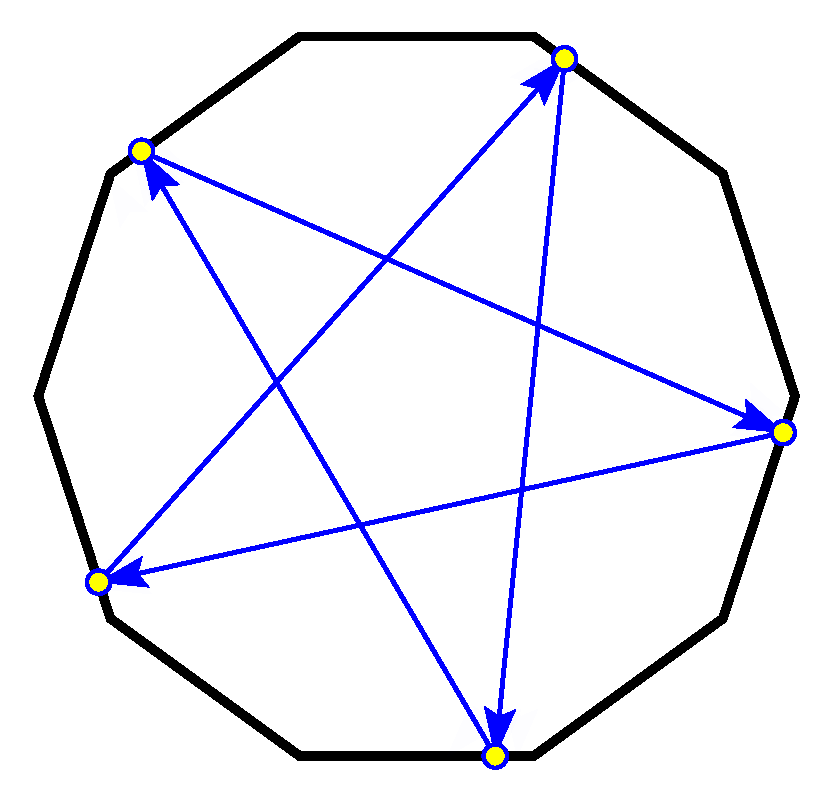
\includegraphics[width=0.7\linewidth]{../figs/nonagon_neg0pt8rad_skip3.pdf}

\end{subfigure}%
\begin{subfigure}{0.25\textwidth}

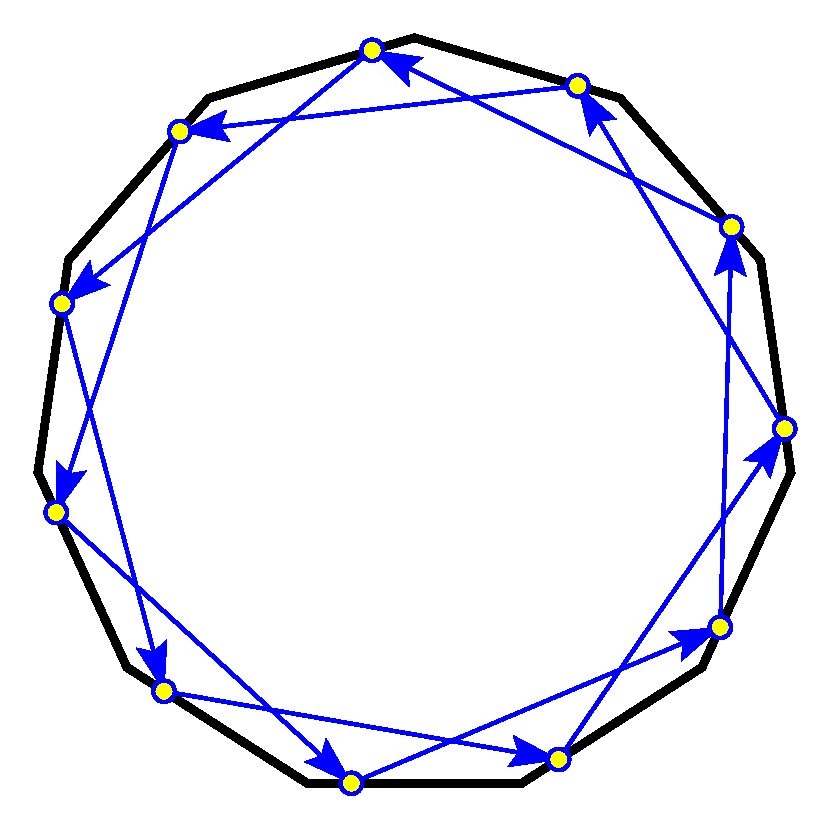
\includegraphics[width=0.7\linewidth]{../figs/eleven_limit_m2.pdf}

\end{subfigure}

\caption{Simulated orbits for generalized edge bouncing in
regular polygons, with $n=9, m=4, \theta=-0.8$ rad and $n=11, m=2, \theta=0.4$
rad. Predicted collision points are indicated by circles. Both simulations are of the trajectory after 300 bounces
from an arbitrary start point. \label{ccw-m-bounce}}
\end{figure}


\subsection{Implications for Uncertainty in Implementations}
All physical implementations of the required motion primitives
will be imperfect - for example, differential drive robots can have asymmetries
in the motors powering each wheel, which can result in a curved path
through the interior of the environment, or an inaccurate rotation
while aligning to $\theta$. These differences between the model and 
the implementation produce a constant offset in the bounce angle, $\theta + \epsilon$. 
Theorem \ref{Theorem:1} gives a bound on the maximum allowable error in this
situation, and suggests that random errors within this bound will still result
in near-periodic orbits.

For each stable orbit in a given environment, we can use the bounds on
$c(\theta)$ to determine the range of angles that will result in that orbit. 
Thus, when designing a ``patrolling" robot in an environment with regular polygonal
geometry, a robot designed to bounce at an angle $\theta$ in the center of one of these
ranges ($ \phi_m/2< \theta < \phi_{m-1}/2$ or $-\phi_{m-1}/2 < \theta <
-\phi_m/2$) will be maximally robust to actuator or sensor errors. The resulting
maximum allowable error, $\epsilon_{max}$, will be $\pm | (\phi_m - \phi_{m-1})/2 |$.
Bounces with error within this range will still result in stable orbits of the
workspace, because the bounce still acts as a contraction mapping on the edge
intervals.

However, these orbits will impact the boundary at
different locations than expected. If there is a constant error in the bounce
angle, so that the effective bounce angle is $\theta + \epsilon$, with $\epsilon
< \epsilon_{max}$, the resulting difference in the location of the collision point
on each edge will be $\Delta_x = b_{m,\theta + \epsilon}^{\infty} - b_{m,\theta}^{\infty}$.


\section{SIMULATIONS}
The figures and experimental simulations for this paper were computed using a
Haskell program which heavily used the
\textit{Diagrams} library \cite{yorgey2012monoids}. 
The simulator can also be used for specular bouncing simulations, and could be
of use to those studying classical billiards, or variants such as pinball billiards.
It is also capable of simulating random bounces, or random noise on top of  
deterministic bouncing. Code is open source and on GitHub
\footnote{\url{https://github.com/alexandroid000/bounce}}.

The purpose of the simulations is to confirm experimentally
the theoretical results obtained in previous sections. Figure~\ref{prediction} 
depicts simulated orbits for adjacent edge bouncing after 300 bounces. 
Predicted collision points $x_{FP}$ are indicated by circles. Figure~\ref{gen_bounce}
shows simulated orbits for two pairs of $n$ and $m$ values in the case where the
robot bounces skipping $m-1$ edges. The trajectories after 300 bounces are displayed.

Note that the simulated orbits were computed by iteratively bouncing
the robot in the environment from an arbitrary start point rather than just
plotting the resulting orbit from the predicted collision points.
In all simulations, the simulated collision points (tips of arrows) and the
theorized collision points $x_{FP}$ (circles) coincide.

Figure~\ref{fig:multi_start} shows three orbits simulated from different 
start points but with the same bouncing angle $\theta$. Regardless of starting
position, the same bouncing angle $\theta$ produces trajectories which
converge to the same limit cycle, as stated in 
Remark~\ref{rm1}.


As stated in Theorem~\ref{Theorem:1} there exist ranges of $\theta$ that 
produce stable orbits when the robot skips $m-1$ edges with $m \geq 1$. For
regular hexagons, $\pi/3$ is the lower bound on $\theta$ such that the
robot strikes every edge sequentially, and the upper bound on $\theta$ such that
the robot strikes every other edge.
The orbits shown in Figure~\ref{fig:multi} were generated setting
$\theta = \pi/3 \pm 0.05$. As predicted, one orbit
bounces off every other edge, while the other strikes every sequential edge.

\begin{figure}[bh]
\begin{subfigure}{.23\textwidth}
\centering

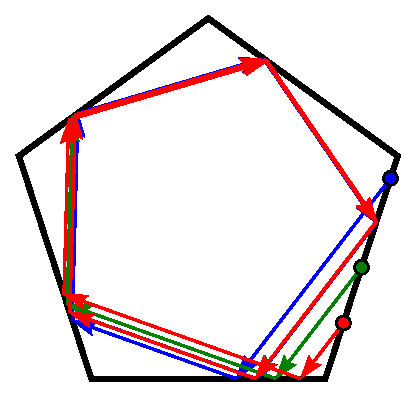
\includegraphics[width=\textwidth]{../figs/multi_start.pdf}
\captionof{figure}{Three orbits simulated with different start points - the three circles - but same bouncing angle $\theta$. The limit cycle is the same.
\label{fig:multi_start}}

\end{subfigure}%
\hfill
\begin{subfigure}{0.23\textwidth}

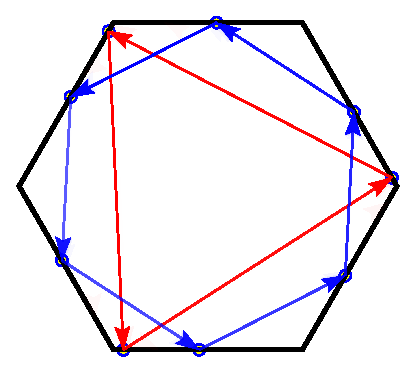
\includegraphics[width=\textwidth]{../figs/multi.pdf}
\captionof{figure}{Two simulated orbits with the same start point but
$\theta$ set to $\pi/3 + 0.05$ (blue) and $\pi/3 - 0.05$ (red). One skips
no edges and the other skips one edge.
\label{fig:multi}}

\end{subfigure}
\caption{Evidence from simulation that (a) limit cycles are independent of start
position, and that (b) our predicted ``transition angle" between
striking every edge and every other edge is correct.}
\end{figure}


%\begin{figure}[bh]
%\centering
%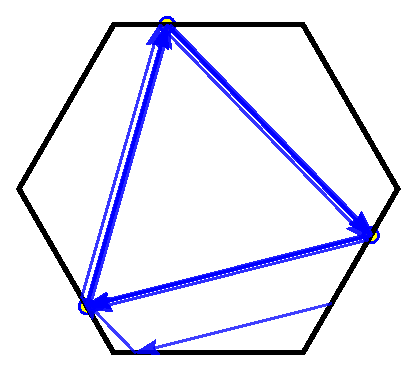
\includegraphics[width=0.2\textwidth]{figs/convergence.pdf}
%\captionof{figure}{A bounce from edge $p_0p_1$ to edge $p_mp_{m+1}$. The other
%edges of the polygon are not drawn.
%\label{fig:conver}}
%\end{figure}

\section{CONCLUSIONS AND FUTURE WORK} \label{conclusion}

In this paper we considered robots that drive in straight 
lines and “bounce” off boundaries at controllable angles. 
We analysed the location and stability of periodic orbits in 
regular polygons, which might be used to patrol the space 
on a repeatable, periodic path.

We first presented the case of stable orbits that bounce 
off each adjacent edge. We proved the existence of periodic
orbits in $n$-sided regular polygons, and showed the range of
bounce angles that will produce such orbits along with an analysis 
of their stability and robustness to modeling errors.
We generalized our results to the case
where the robot skips $m-1$ edges. 
In both cases we present a closed form solution for the locations
where the robot collides with the environment boundary while 
patrolling. 

The existence of periodic orbits along with the presented 
closed form solutions for $x_{FP}$ show that it is possible to 
design a robust patrolling path for a given environment, using limited motion
and sensing capabilities. These orbits
have the useful properties of being robust to modelling errors and being
independent of the start position.

One interesting line of research could be to explore how the convergence of
these orbits could be used to narrow down the set of possible positions of the
robot, in navigation and localization tasks.

\begin{figure}[t]
\begin{subfigure}{.23\textwidth}
\centering
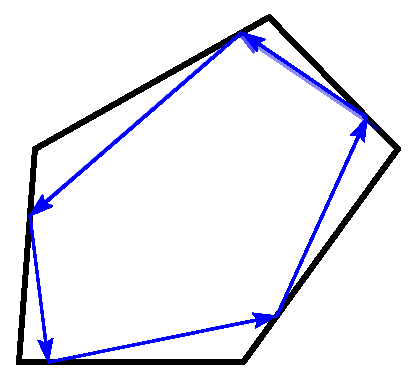
\includegraphics[width=0.8\linewidth]{../figs/shear.pdf}
\caption{A stable orbit in a sheared pentagon.}
\label{shear}
\end{subfigure}%
\hfill
\begin{subfigure}{0.23\textwidth}
\centering
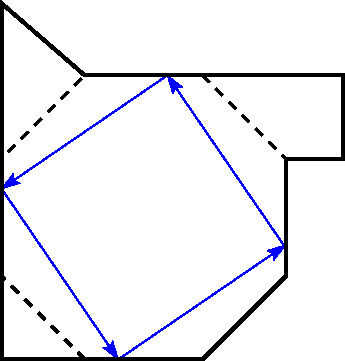
\includegraphics[width=0.6\linewidth]{../figs/oct.pdf}
\caption{A stable orbit in a nonconvex environment.}
\label{oct}
\end{subfigure}
\caption{Stable orbits also exist in non-regular polygons. }
\label{squish-shear}
\end{figure}

The most pressing open question is how to extend the current analysis to 
non-regular polygons. In non-regular polygons, it is not clear how to 
solve for orbits as the fixed point of one
mapping function. Yet, limit cycles still exist in other polygons, such as
regular polygons under linear transformations, as seen in Figure \ref{shear}.
It is worth mentioning that our current analysis can be used to design stable
orbits in polygons with enough local similarity to regular polygons, such
as in Figure \ref{oct}.

Another direction for future research is to consider a 
time-varying error $\epsilon(t)$ over $\theta$. This would
allow us to model external disturbances to the 
motion and sensing of the robot. In
simulations we have noticed that if $\epsilon(t)$ does not cause $\theta \pm
\epsilon(t)$ to exceed the bounds on $\theta$ that cause periodic orbits, the robot's 
trajectory stays within a certain range of the predicted collision points. 
A theoretical analysis of these observations would be useful. 

\addtolength{\textheight}{-12cm}   % This command serves to balance the column lengths
                                  % on the last page of the document manually. It shortens
                                  % the textheight of the last page by a suitable amount.
                                  % This command does not take effect until the next page
                                  % so it should come on the page before the last. Make
                                  % sure that you do not shorten the textheight too much.

%%%%%%%%%%%%%%%%%%%%%%%%%%%%%%%%%%%%%%%%%%%%%%%%%%%%%%%%%%%%%%%%%%%%%%%%%%%%%%%%



%%%%%%%%%%%%%%%%%%%%%%%%%%%%%%%%%%%%%%%%%%%%%%%%%%%%%%%%%%%%%%%%%%%%%%%%%%%%%%%%



%%%%%%%%%%%%%%%%%%%%%%%%%%%%%%%%%%%%%%%%%%%%%%%%%%%%%%%%%%%%%%%%%%%%%%%%%%%%%%%%

\section*{ACKNOWLEDGMENT}

This work is supported by NSF grant 1035345, NSF grant 1328018, and CONACyT
post-doctoral fellowship 277028. The authors would like to thank Michael Zeng
for his contributions to the fixed-point formulation of the problem.

%%%%%%%%%%%%%%%%%%%%%%%%%%%%%%%%%%%%%%%%%%%%%%%%%%%%%%%%%%%%%%%%%%%%%%%%%%%%%%%%

\bibliographystyle{IEEEtran}
\bibliography{IEEEabrv,refs}





\end{document}
